\subsection{Gene Ontology Visualization}
\label{sec:go}

Gene Ontology graph is a directed acyclic graph and highly connected: 24,153 edges and 10,041 vertices, where 3,918 are unconnected components.
Figure~\ref{fig:go_connections_yEd} shows how extremely connected the graph is, the picture was produced by yEd graph editing tool.

\begin{figure}
\centering
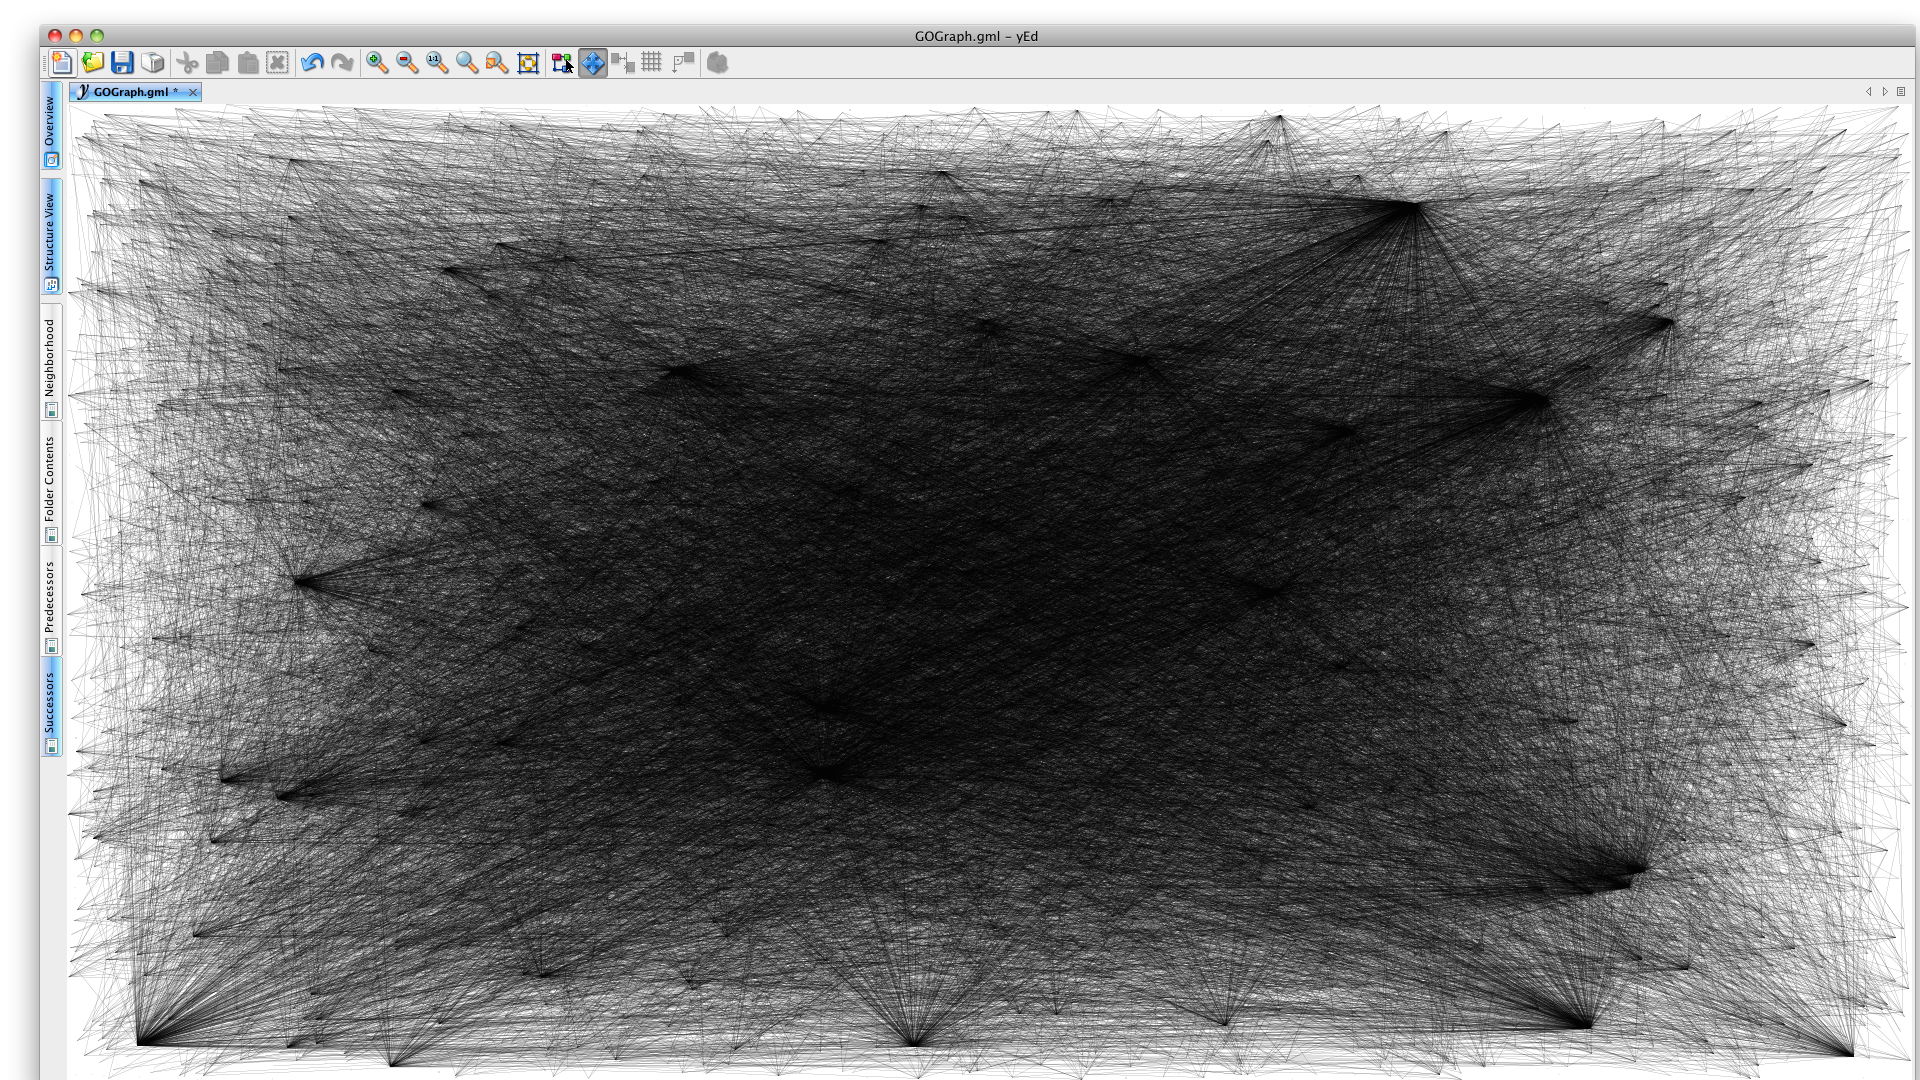
\includegraphics[scale=0.2]{pictures/yEd_GO_2.png}
\caption{Gene Ontology graph visualization using yEd}
\label{fig:go_connections_yEd}
\end{figure}

The high connectivity between elements in the source graph makes it very complicated to explore. Provided visualization approach has several goals.
The first goal is to reduce amount of connections between vertices by showing edges only for ``current'' sub-graph.
It allows to see where the sub-graph is aligned in the whole graph and, in the same time, helps to track it's inner structure.
Second goal is an ability to switch from working with genes of the GO graph to discovering relations between GO and Cluster graphs.
For this purpose there are two view modes for GO graph:

\begin{itemize}
   \item levels overview --- show graph levels from top to bottom with corresponding content as ``preview'';
   \item zoomed view --- visualizes only on three levels at the same time in order to focus on genes inside;
\end{itemize}

The last but not least goal is to explicitly show nodes and leaves. Each level is divided into two sections where leaves are red colored on the left and node genes are on the right and having white color.
Color schema can be changes through the settings menu but not leaves-nodes location.
This feature gives further insight into the topology of a specific layer by gaining information about the distribution of leaves and nodes on a particular layer.

There are two layout implementations based on the goals discussed before. First GO layout is ``Levels Layout'' and is shown in Figure~\ref{fig:go_levels_layout}.
Genes are ordered by layers depending on their graph-theoretic distance from the root.

\begin{figure}[h!]
\centering
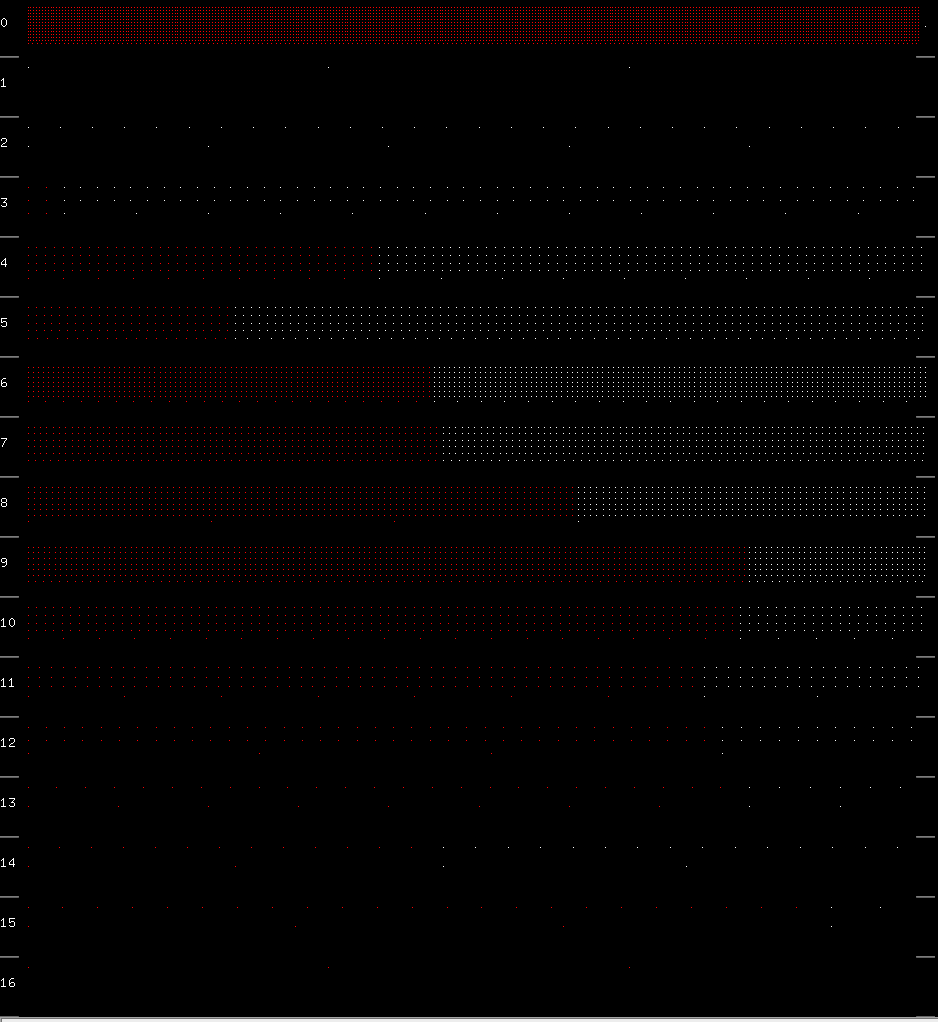
\includegraphics[scale=0.3]{pictures/go_levels_layout.png}
\caption{Gene Ontology Levels Layout visualisation}
\label{fig:go_levels_layout}
\end{figure}

Figure~\ref{fig:go_levels_layout_zoomed} displays the situation when the user zooms in the view.
Although the resulting visualization looks like bar charts, the number of leaves cannot be precisely compared between different layers since
the area the red node pixels (leaves) cover is not proportional to the total number of leaves in each layer.
However, it is proportional to the sum of nodes in that particular layer. In other words, the covered area depends on the specific layer density.
There are unconnected components in the Gene Ontology graph.
Unconnected nodes are placed in the top layer number --- zero. There is an option to show-hide unconnected components from the main menu.
The spatial arrangement of the node pixels within a layer, except the placing of leaves and nodes are in specific regions, is random.

\begin{figure}[h!]
\centering
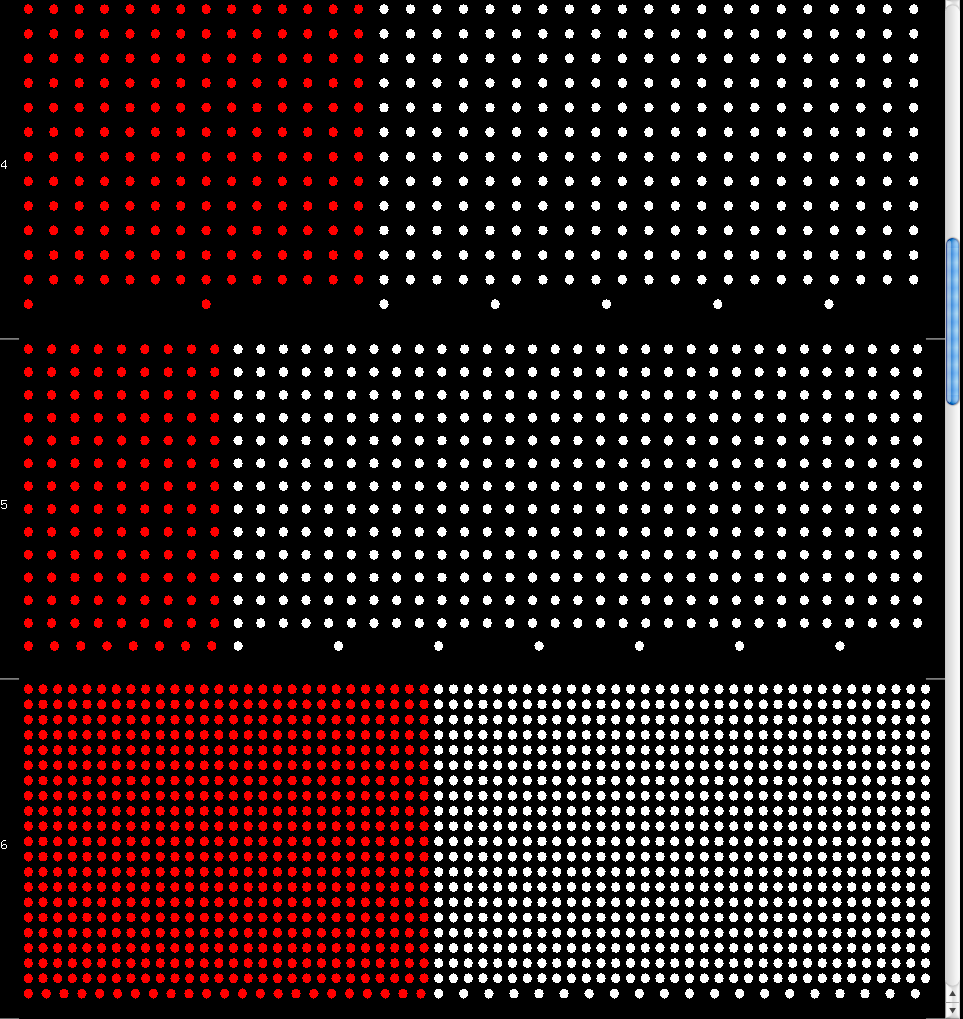
\includegraphics[scale=0.3]{pictures/go_levels_layout_zoomed.png}
\caption{Zoomed view}
\label{fig:go_levels_layout_zoomed}
\end{figure}

Second layering approach ``Leaves Bottom Layout''
(Figure~\ref{fig:go_leaves_bottom_layout}) is similar to the first one in terms of placing the nodes into corresponding layers based on the distance
from the source node and random distribution of the node pixels within each layer.
However, all leaves are placed into one single layer together with unconnected nodes at the bottom of the GO view, i. e., in the layer with the highest number.
Unconnected nodes can be filtered out if necessary. This approach gives insight into the distribution of nodes among different layers without the distraction of the leaves,
thus enriching the perception of the graph topology.

\begin{figure}[h!]
\centering
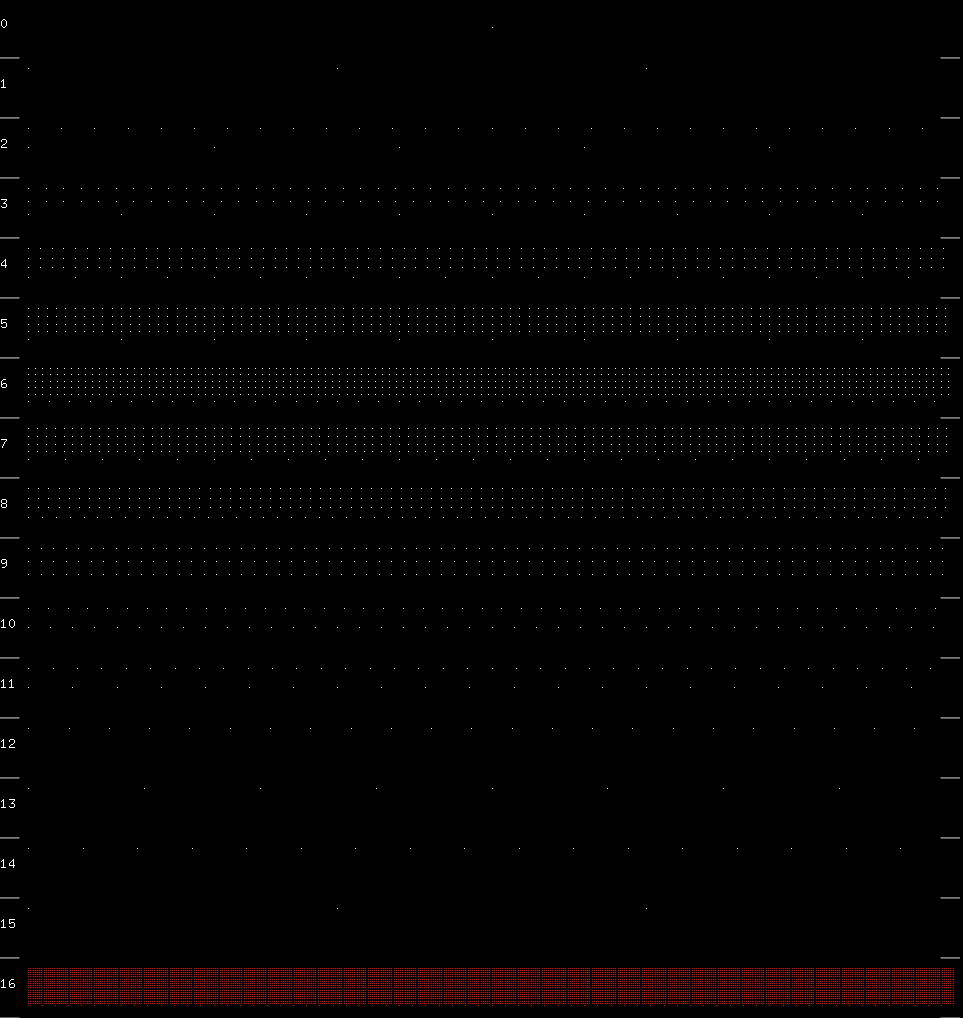
\includegraphics[scale=0.3]{pictures/go_leaves_bottom_layout.png}
\caption{Leaves bottom layout}
\label{fig:go_leaves_bottom_layout}
\end{figure}

All provided features help to improve visualization and decrees amount of element in the scene. But even with hided edges visualized sub-tree could be complicated.
The result of sub-graph highlighting is shown in Figure~\ref{fig:go_no_edge_bundling}.

\begin{figure}[h!]
\centering
\subfloat[Straight edges]{
    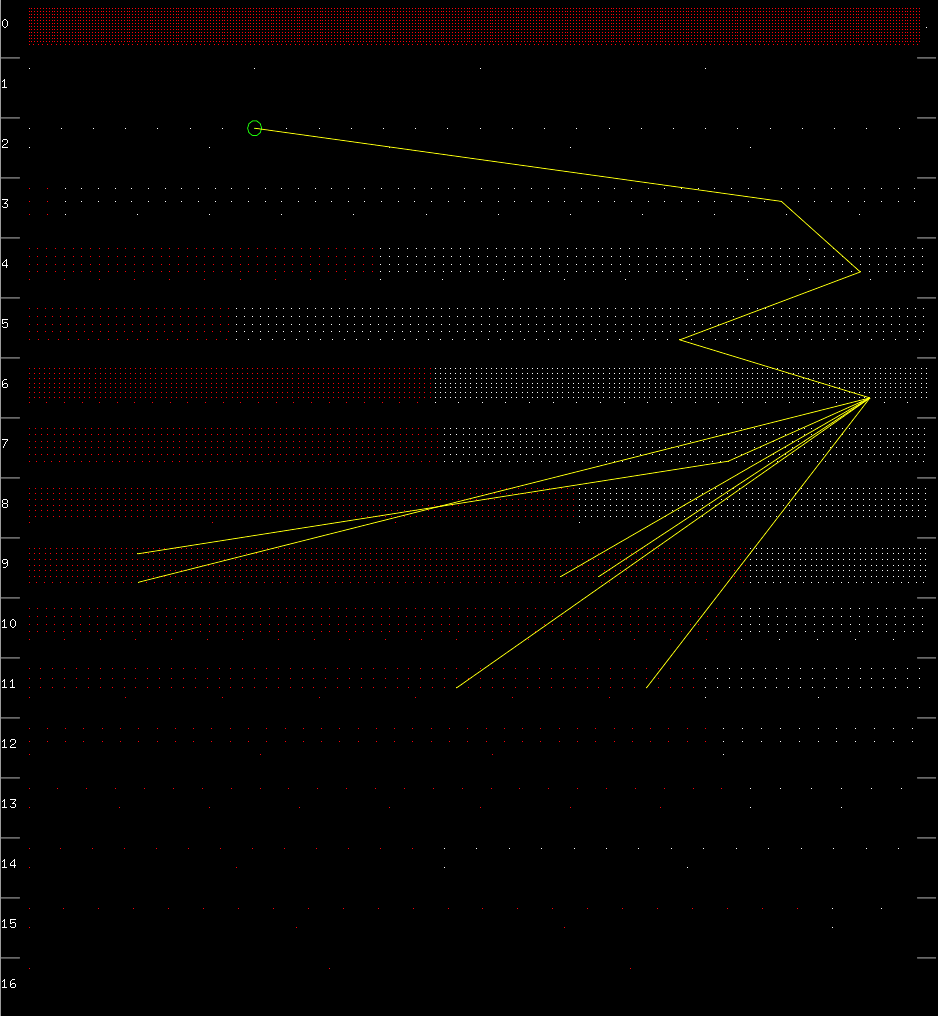
\includegraphics[scale=0.2]{pictures/go_no_edge_bundling.png}
    \label{fig:go_no_edge_bundling}
}
\subfloat[Edge bungling]{
    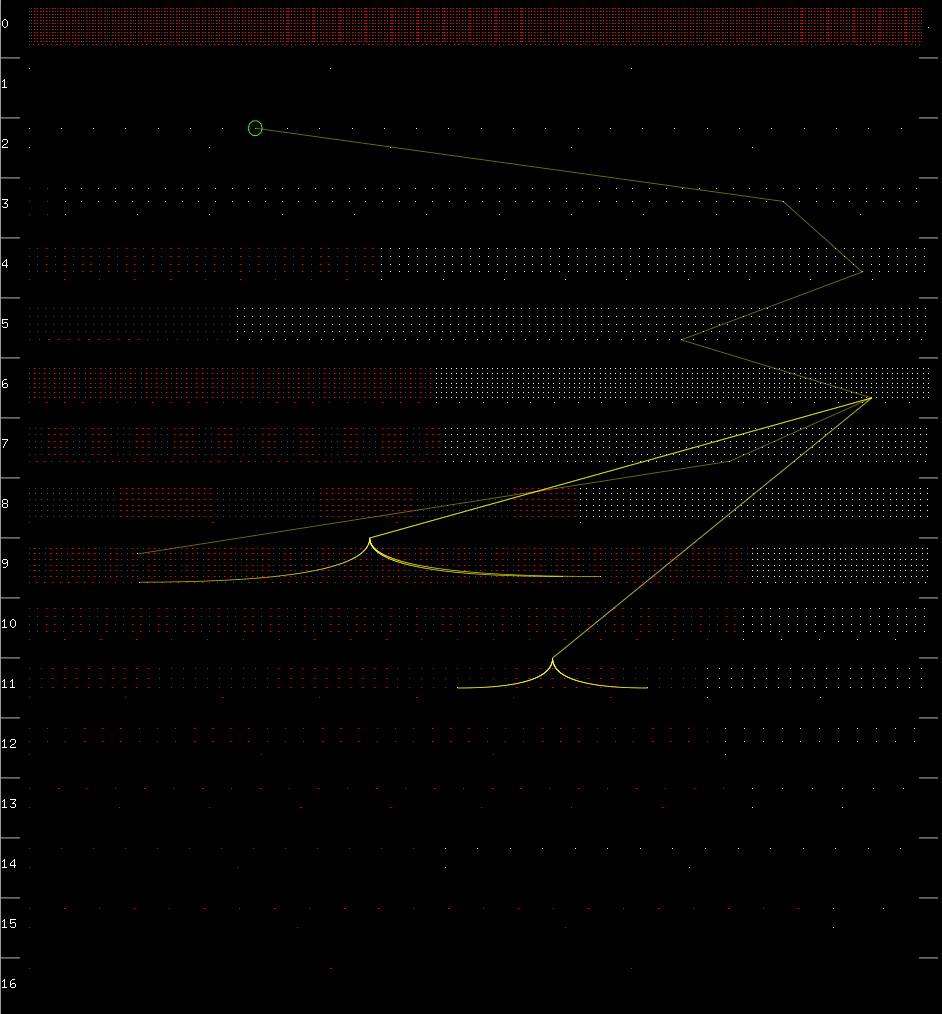
\includegraphics[scale=0.2]{pictures/go_edge_bundling.png}
    \label{fig:go_edge_bundling}
}
\caption{Gene Ontology sub-graph edge highlighting}
\label{fig:go_subgraph_highlighting}
\end{figure}

Improved edge visualization for the same selected vertex ``multicellular organismal process'' is shown in Figure~\ref{fig:go_edge_bundling}.
A newer solution is simple edge bundling. Edge bundling technique and usage example well described in the~\cite{EDGE_BUNDLING_1} and~\cite{EDGE_BUNDLING_2}.

For all edges which go into same level computed ``dummy node'' located on the top of the target level and in the middle of outlined vertices, drawing single line from source to
``dummy node'' as first part. Second part is to draw ``Bezier line'' from ``dummy node'' to target vertex. This solution helps to follow the connection and to use space in the right way.